\section{Geschichtliche Entwicklung von AMT-Systemen}

\subsection{Moorer und das erste AMT-System}
Eine der ersten Arbeiten über automatische Musiktranskription wurde im Jahr 1977 geschrieben \cite{Moorer1977}.
In dieser beschreibt Moorer seinen Ansatz, polyphone Musikaudiospuren
direkt über Computerprogramme in Notenschrift zu übertragen.
Während dieses Prozesses fallen ihm schon große Probleme auf, die auch in späteren Arbeiten
eine ausschlaggebende Rolle spielen.

\subsubsection{Grundlegende Probleme}
Eines dieser Probleme wird von ihm als das \enquote{Cocktail-Party-Problem} bezeichnet.
Dieses stellt die Schwierigkeit dar, auf einer Party bestimmten Stimmen zu folgen, während viele verschiedene Stimmen
gleichzeitig erklingen.
Das gleiche Problem existiert in der Noten transkription.
Die meisten Musikstücke haben mehrere Instrumente, welche gleichzeitig spielen.
Oft gibt es auch Musikstücke, bei denen es mehrere Stimmen für ein Instrument gibt.
Ein Beispiel dafür ist die Violine, die zum Beispiel in Orchesterstücken oft auf mehrere Stimmen (erste, zweite, dritte) aufgeteilt wird.
Dies erschwert die Zuordnung bestimmter Noten zu einer gewählten Stimme.
Der Großteil aller Menschen scheitert daran große Musikstücke richtig zu transkribieren.
Noch schwieriger wird es für Computerprogramme.
Anfangs identifizieren diese bestimmte Töne anhand der Frequenz des Tons.
Moorer stellte fest, dass sich allein anhand der Frequenz nicht eindeutig bestimmen lässt,
welche Töne zu einem bestimmten Zeitpunkt gespielt werden.

Das nächste Problem ist die Frequenzüberladung durch Obertöne.
Jeder Ton hat Obertöne.
Diese Obertöne sind jeweils das Vielfache des gespielten Grundtons.
Wird beispielsweise auf einem Klavier der Ton C3 (130,81 Hz) gespielt,
so entstehen die Obertöne C4 (261,62 Hz), G4 (392,42 Hz) und weitere.
Auch wenn nur C3 gespielt wird, erkennt das Computerprogramm zusätzlich die jeweiligen Obertöne,
was als Frequenzüberlagerung bezeichnet wird.
Diese Frequenzüberlagerung sorgt dafür, das zum Beispiel ein Klavier anders klingt als eine Violine.
Daraus resultiert die Klangfarbe (Timbre) eines bestimmten Instrumentes \cite{goswami2013timbre}.
Moorer konnte das Problem der Obertöne nicht lösen.
Zum einen war es ihm aufgrund des damaligen technischen Stands nicht möglich, die Klangfarbe eines Instruments zu erkennen.
Zum anderen waren die Algorithmen und Verfahren jener Zeit nicht in der Lage, die Grundfrequenz von den Obertönen zu trennen.
Deshalb fokussierte er sich ausschließlich auf zweistimmige polyphone Musikstücke.

Ein weiteres Problem war Rauschen in unter realen Aufnahmebedingungen erstellten Audiospuren
sowie stilistische Mittel in der Musik, wie etwa Vibrato.
In real aufgenommenen Audiospuren gibt es immer ein gewisses Hintergrundrauschen \cite{iZotope2025noisefloor}.
Dieses kann von einem Computerprogramm auch als Note erkannt werden oder verhindern,
dass bestimmte Noten richtig erkannt werden.
Moorer nahm das Musikstück selbst analog auf und digitalisierte es anschließend mit einem 14-Bit-A/D-Wandler.
Durch die eigene Aufnahme konnte er die Aufnahmeumgebung, die Mikrofonposition
und die genutzte Technik kontrollieren, wodurch sich das Rauschen im Vergleich zu unkontrollierten Aufnahmen verringerte.
Zudem wies er die Musiker an auf stilistische Mittel zu verzichten.
Stilistische Mittel wie Vibrato verursachen kleine, aber kontinuierliche Veränderungen der Frequenz.
Dadurch kann das Computerprogramm nicht korrekt erkennen, das eigentlich eine einzelne Note gespielt wurde.
Die Folge davon wäre eine falsche Zuordnung des Onsets und Offsets der Noten.
Ohne diese erhielt Moorer klarere und besser verwertbare Daten für die Transkription.

Das letzte Problem, was Moorer angesprochen hat, ist die Nutzung von nicht
harmonischen Instrumenten wie Trommeln oder einem Schlagzeug.
Diese Instrumente haben keinen eindeutigen Pitch.
Sie sind abhängig von dem Rhythms und der Lautstärke.
Da Moorers AMT sich jedoch auf das Frequenzmuster der Noten fokussiert,
konnten diese Musikinstrumente nicht berücksichtigt werden.

\subsubsection{Der Aufbau von Moorers AMT-System}
Moorers automatische Musiktranskriptionssystem war eins der ersten seiner Art.
Viele weitere AMT-Systeme leiten sich von diesem ab.

Zunächst wird ein analoges Musiksignal mit einem 14-Bit-A/D-Wandler digitalisiert.
Dieses digitale Musiksignal wurde anschließend genutzt, um mithilfe von Bandpassfiltern,
bestimmte Frequenzbereiche zu isolieren.
Ein Bandpassfiltern ist ein Filter welcher nur bestimmte Frequenzen durchlässt.
Dadurch konnte Moorer die gespielte Note und deren Dauer,
wie deren Onset und Offset, feststellen.

Nun mussten die bestimmten Noten einer gewählten Stimme zugeordnet werden.
Dies wurde durch melodische Gruppierung verwirklicht.
Zunächst wurden Inseln gebildet.
Inseln sind Noten die sich Zeitlich vollständig überlappen.
Wir gehen davon aus das jede Stimme nur eine Note gleichzeitig spielt,
wodurch diese Noten nicht der gleichen Stimme zugeordnet werden können.
Als Nächstes müssen die anderen Noten auf verschiedene Kombinationen getestet werden.
Je geringer die Frequenzunterschiede zwischen aufeinanderfolgenden Noten sind,
desto wahrscheinlicher stammen sie aus derselben Stimme.
Dies liegt daran, dass melodische Linien in der Regel durch kleine, schrittweise Intervalle fortgeführt werden,
während größere Sprünge häufiger auf einen Wechsel der Stimme hindeuten.
Zudem werden Gruppierungen von Noten erstellt, welche am wahrscheinlichsten harmonisch nacheinander gespielt worden.

Zum Schluss ließ Moorer die gewonnenen Daten durch ein Programm laufen, 
um diese dann mithilfe eines Plotters in eine Notenschrift umzuwandeln.

\subsection{Hidden Markov Modelle}\label{subsec:hiddenMarkov}
Hidden Markov Modelle (HMM) sind statische Modelle, welche sich sehr gut zur Analyse von Musikstücken eignen.
Sie wurden erstmals in den 1960er Jahren erfunden \cite{baum1970maximization} und
sind ein zentraler bestandteil früher AMT-Systeme.
HMMs beschreiben eine Abfolge von \enquote{versteckten Zuständen},
welche im Kontext von AMT-Systemen Noten im Audiosignal darstellen.
Durch indirekt beobachtbare Daten, wie zum Beispiel die Spektraldaten des Audiosignals,
können diese Noten erschlossen werden.

HMMs bestehen aus:
\begin{itemize}
    \item Zustände (States)
    \item Übergangswahrscheinlichkeiten (Transition Probabilities)
    \item Emissionswahrscheinlichkeiten (Emission Probabilities)
    \item Beobachtungen (Observations)
\end{itemize}
Nehmen wir das Beispiel eines Klaviers.
Ein Klavier hat 88 Tasten, und somit mindestens 88 Zustände.
Durch Akkorde können zudem mehr Zustände generiert werden.
Die Übergangswahrscheinlichkeit stellt dar,
wie wahrscheinlich es ist, von einem Zustand zu einem bestimmten anderen Zustand zu wechseln.
Zum Beispiel könnte es wahrscheinlicher sein, dass auf die Note C4 der Ton G3 folgt statt D1,
da diese Tonfolge harmonischer und musikalisch plausibler klingt.
Dies ist jedoch nur eine Annahme anhand von gesammelten Testdaten, weshalb es nicht als Begründung ausreicht.
Deshalb kommt als zweite Instanz die Emissionswahrscheinlichkeit hinzu.
Diese gibt an, wie wahrscheinlich ein bestimmter Zustand in der momentanen Beobachtung ist.
Die Beobachtung wird dabei aus Eigenschaften wie Frequenzverteilung,
Spektrogramm oder anderen Merkmalen zusammengesetzt, die aus verschiedenen Modulen hergeleitet werden können.
Aus den gesammelten Daten kann nun mithilfe von zum Beispiel dem Viterbi-Algorithmus \cite{takeda2002hidden} die
wahrscheinlichste Abfolge von Zuständen berechnet werden.

In gewisser Weise lassen sich HMMs auf KI-Modelle übertragen.
Beide arbeiten mit versteckten Zuständen und
berechnen anhand von Testdaten die wahrscheinlichste Kombination von Zuständen.
Natürlich sind moderne KI-Modelle weitaus komplexer,
doch HMMs spielten im Kontext automatischer Musiktranskriptionssysteme eine zentrale Rolle dabei,
wie KI-Methoden in diesem Bereich später eingesetzt wurden.
Sie beeinflussten insbesondere den Umgang mit zeitlichen Abfolgen
und Unsicherheiten in der Tonerkennung,
was bis heute relevante Konzepte in KI-basierten AMT-Systemen sind.

\subsection{Datensätze für AMT-Systeme}
Während der Forschung an neuen AMT-Systemen wurden immer wieder neue Datensätze genutzt,
um AMT-Systeme zu bespielen oder heutzutage auch zu trainieren.
Es ist aufwändig nützliche Datensätze zu generieren,
da viele verschiedene Musikstücke genutzt werden müssen und diese alle unter den gleichen Voraussetzungen aufgenommen werden müssen.
In der Transkription von Musikstücken sind Datensätze sehr relevant,
vor allem mit dem weiteren Einsatz von KI-Modellen werden große Datensätze gebraucht.
Die ersten verwendeten Datensätze waren selbst erstellt und enthielten lediglich grundlegende Eigenschaften der Noten.
In den AMT-Systemen von Moorer \cite{Moorer1977} oder auch Martin \cite{Martin1996} wurde solch ein Ansatz verfolgt.
Durch die Einführung von MIDI-Dateien wurde ein Standard entwickelt,
welcher jetzt im Großteil der AMT-Systeme eingebaut wird.
Auf der Grundlage von MIDI-Dateien wurden auch spezialisierte Datensätze erstellte.
Zwei der größten und wichtigsten sind MAPS (MIDI Aligned Piano Sounds) und
MAESTRO (MIDI and Audio Edited for Synchronous Tracks and Organization).
Dabei ist MAPS ein Datensatz aus künstlich generierten Audiospuren,
während MAESTRO ein ungefähr 200 Stunden langer Datensatz von realen isolierten Studioaufnahmen ist.
Vor allem bei dem Training neuer KI-Modellen sind solche großen Datensätze sehr hilfreich.
Ein weiterer wichtiger Datensatz ist ADTOF (Annotated Drum Transcription Onset Features).
Dieser besteht ausschließlich aus unharmonischen Instrumenten.
In Moorers und anderen AMT-Systemen ist die Erkennung von unharmonischen Instrumenten ein großes Problem.
KI-Modelle können sich mithilfe von dem ADTOF Datensatz auf diese Instrumente spezialisieren.
Es gibt auch Methoden schnell seine eigenen Datensätze zu generieren.
Eine der neuesten Methoden verwendet HMM- und Viterbi-basierte Alignment-Verfahren,
um synthetische Audiosignale zu erzeugen und so zusätzliche Daten für das Training
von KI-Modellen bereitzustellen \cite{joysingh2019development}.

\subsection{Polyphone AMT-Systeme}
Die meisten früheren AMT-Systeme befassten sich mit monophonen Musikstücken oder höchstens zweistimmigen Ansätzen.
Der Großteil realer Musikwerke ist jedoch polyphon, das heißt, es erklingen mehrere Stimmen gleichzeitig.
Die Polyphonie stellte und stellt bis heute eine der größten Herausforderungen der automatischen Musiktranskription dar.
Sie bringt zahlreiche Probleme mit sich, etwa komplexere Spektrogrammmuster, höheren Rechenaufwand und überlappende Stimmen.
Eine Lösung für polyphone Musikstücke markierte daher einen wichtigen Meilenstein in der Entwicklung von AMT-Systemen.
Aus diesem Grund widmeten sich mehrere Forscher dieser Fragestellung und entwickelten innovative Ansätze,
wie etwa das Blackboard-System oder RASTA-basierte AMT-Systeme, die in diesem Kapitel vorgestellt werden.

\subsubsection{Blackboard-System}
Zunächst wird das Martin AMT-System \cite{Martin1996} vorgestellt.
Sein Ansatz, zur Lösung von polyphonen Musikstücken, war ein Blackboard-System.
Dieses integrierte er in sein AMT-System mit innovativen Modulen und Ansätzen.

Zur Verarbeitung des Input Audiosignals nutzt Martin ein Correlogram.
Im Gegensatz zum Spektrogramm, das die Energieverteilung über Frequenzen zeigt,
hebt das Correlogram durch Autokorrelation vor allem periodische Strukturen und Tonhöhen hervor.
Nachdem das Input Audiosignal in einem Correlogram verarbeitet wurde,
spaltet sich Martins AMT-System, in einen Analysepfad und einen Rhythmuspfad, auf.
Dabei konzentriert sich der Analysepfad auf die Zusammenhänge der verschiedenen Noten,
während der Rhythmuspfad sich mit der Lautstärke und den Notenanschlägen beschäftigt.
Am Ende werden diese Kenntnisse zusammengeführt.
Der Output besteht aus dem Onset, der Dauer und der Frequenz jeder gespielten Note.
Martins AMT-System gibt nicht explizit zurück, welcher Stimme jede Note zugeordnet ist.
Durch das Blackboard-System und insbesondere durch die sequentielle Analyse der Intervalle
lassen sich die erkannten Noten nachträglich den einzelnen Stimmen korrekt zuordnen.

\begin{figure}[H]
    \centering
    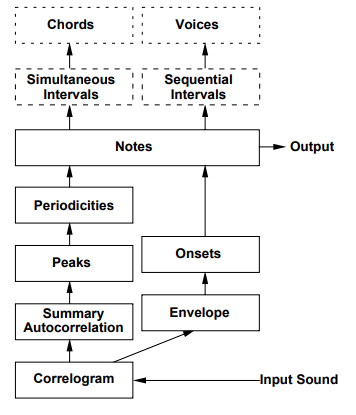
\includegraphics[width=0.6\textwidth]{Graphics/Martin1996Structure}
    \caption[Systemstruktur nach Martin]{Systemstruktur des AMT-Ansatzes von Keith D. Martin (1996), aus  \cite{Martin1996}.}
    \label{fig:martin-structure}
\end{figure}

Martin nutzt ein Blackboard-System.
Dieses besteht aus zwei Hauptbestandteilen.
Der erste Teil ist die Sinuskurvenanalyse, mit der die für die Hypothesenbildung notwendigen Daten gewonnen werden.
Zu ihr gehören das Correlogram, das Envelope, die Summary Autocorrelation und die Peaks.
Durch diese Verarbeitungsschritte können zentrale Eigenschaften der Noten bestimmt werden,
die als Grundlage für weitere Analysen dienen.

Zum zweiten Teil gehören die Module Onsets, Periodicities sowie Simultaneous und Sequential Intervals.
Diese Module arbeiten kollaborativ auf einem gemeinsamen Datenraum,
indem sie Hypothesen über die ermittelten Noten aufstellen und sich gegenseitig mit zusätzlichen Informationen versorgen.
Auf diese Weise lassen sich die erkannten Noten später einzelnen Stimmen zuordnen.

Der Analysepfad beginnt bei dem Correlogram.
Hier wird der Input, ein reales Audiosignal,
zunächst verarbeitet und dann in einem Correlogram dargestellt.
Dieses visualisiert die Korrelation der gegebenen Noten in Abhängigkeit der Zeit, Frequenz und Verzögerung.
Die Verzögerung soll in diesem Fall darstellen, wann sich ein bestimmtes Signal wiederholt.
Dabei ist das wiederholte Signal dasjenige, das dem Ursprungssignal maximal ähnelt,
was bedeutet, dass der Korrelationswert an dieser Stelle am höchsten ist.
Heißt, wenn ein Ton mit der Frequenz $x$ gespielt wird
und dieser sich nach beispielsweise 10ms wiederholt, wird das rechnerisch durch die Verzögerung dargestellt.
Als Nächstes wird mithilfe der Summary Autocorrelation das Correlogram komprimiert
und die Datenstruktur normalisiert.
Dadurch entsteht eine stabile Grundfrequenz,
sodass die weiteren Schritte das Correlogram effizient untersuchen können.
Nun werden, basierend auf der normierten Struktur, die Peaks gesucht.
Diese Peaks deuten darauf hin, wann periodische Komponenten auftreten.
Dabei geben sie nicht den Onset der Noten zurück, sondern nur die generelle Frequenz zu einer bestimmten Zeit.
Darauf werden mehrere Peaks, die regelmäßig wiederkehren, gruppiert.
So können Muster in der gespielten Musik erkannt werden und kurzzeitige Störfaktoren ausgeschlossen werden.

Im Rhythmuspfad wird wiederum die zeitliche Analyse der Noten durchgeführt.
Zunächst wird mit dem Envelope die Lautstärke des Signals zu jedem Zeitpunkt festgelegt.
Dies dient als Grundlage, um anschließend die Onsets der Noten zu bestimmen.
Jeder Onset wird präzise im Envelope, durch einen plötzlichen Anstieg der Lautstärke, dargestellt.

Nachdem die beiden Pfade durchlaufen wurden, liegen bereits Noten vor,
die grundsätzlich in Notenschrift transkribiert werden können.
Musikalisch sind diese Noten jedoch noch nicht interpretiert.
In der Abbildung-\ref{fig:martin-structure} gibt es noch die Bestandteile Simultaneous und Sequential Intervals.
In dem Modul Simultaneous Intervals wird ermittelt, welche Töne gleichzeitig erklingen.
Diese können, wenn sie harmonisch zueinander sind, zu einem Chord gebunden werden.
Sequential Intervals analysieren dahingegen, welche Töne nacheinander gespielt werden und
möglicherweise eine Melodie bilden könnten.
Dies erfolgt durch Tonhöhenverläufe, Pausen und Frequenzunterschiede.
Dadurch können Melodien, Basslinien oder Begleitungen voneinander getrennt werden.
Zum Schluss werden dadurch die verschiedenen Stimmen aufgetrennt.

\subsubsection{RASTA-basiertes System}
Ende 1997 publizierte Klapuri seine Masterarbeit \enquote{Automatic transcription of Music} \cite{klapuri1998automatic}.
In seiner Arbeit benutzt er ein neues RASTA-basiertes Verfahren, zur Unterdrückung nicht harmonischer Signalkomponenten.
Somit konnten auch Musikstücke mit nicht harmonischen Instrumenten, wie Trommeln, transkribiert werden.
Zudem führte er ein Modul ein, zur Schätzung der Anzahl an gleichzeitigen Stimmen, die in dem Musikstück vorkommen.
Klapuris AMT-System konzentriert sich, im Gegensatz zu Martins AMT-System, mehr auf die Robustheit gegenüber
echten polyphonen Audioaufnahmen mit Rauschen, Störgeräuschen und nicht harmonischen Instrumenten.
Die Struktur des Systems ist linear aufgebaut und präzise in dem Aufgabenfeld, für die es entwickelt wurde.

\begin{figure}
    \vspace{1em}
    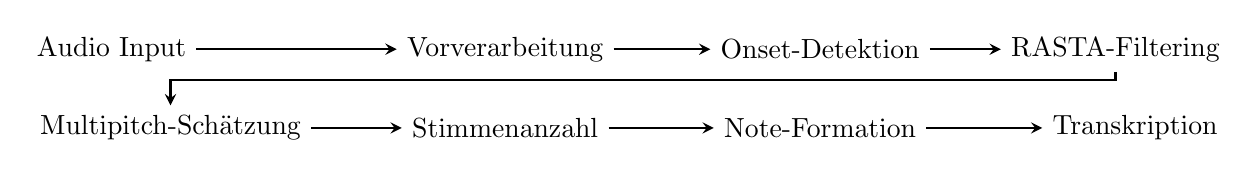
\begin{tikzpicture}[>=stealth, thick]

        % Obere Zeile
        \node at (0,0) (input) {Audio Input};
        \node at (5,0) (prep) {Vorverarbeitung};
        \node at (9,0) (onset) {Onset-Detektion};
        \node at (12.75,0) (rasta) {RASTA-Filtering};

        % Untere Zeile
        \node at (0.75,-1) (multi) {Multipitch-Schätzung};
        \node at (5,-1) (voice) {Stimmenanzahl};
        \node at (9,-1) (notes) {Note-Formation};
        \node at (13,-1) (output) {Transkription};

        % Pfeile obere Zeile
        \draw[->] (input) -- (prep);
        \draw[->] (prep) -- (onset);
        \draw[->] (onset) -- (rasta);

        % Übergangspfeil
        \draw[->] (rasta.south) -- ++(0,-0.1) -| (multi);

        % Pfeile untere Zeile
        \draw[->] (multi) -- (voice);
        \draw[->] (voice) -- (notes);
        \draw[->] (notes) -- (output);

    \end{tikzpicture}
    \vspace{1em}
    
    \label{fig:klapuri_rasta}
    \caption[Struktur eines RASTA-basiertem AMT-System]{Eigene Darstellung: Struktur von Klapuris RASTA-basiertem AMT-System}
\end{figure}

Klapuris System ist sequentiell aufgebaut und besteht aus sechs Modulen.
Als Input wird eine reale Audioaufnahme genutzt, welche in ein Monosignal umgewandelt wird.
Dieses Monosignal wird mithilfe von STFT transformiert,
sodass durch das entstandene Spektrogramm Zeit,
Frequenz und Amplitude der gegebenen Noten ausgelesen werden kann.
Anhand dieser Daten werden als Nächstes die Onsets der Noten bestimmt.
Klapuri nutzt zur Onset-Erkennung ein Schema von Eric D. Scheirer \cite{scheirer1998tempo}.
Dabei wird das Audiosignal in Frequenzbänder aufgeteilt und in jedem Band die zeitliche Änderung der Energie,
die sogenannten \enquote{Energie-Deviate}, berechnet.
Anschließend werden die resultierenden Energieänderungen der verschiedenen Bänder summiert.
Die nun entstehenden Peaks werden als Onsets der Noten interpretiert.
Als Nächstes werden unharmonische Instrumente und transiente Geräusche, wie zum Beispiel Rauschen, entfernt.
Dies erfolgt mithilfe der RASTA-Filterung, welches auf das spektrale Signal, vom gegeben Spektrogramm, wirkt.
Mehr zu der RASTA-Filterung wird im folgenden Abschnitt, \enquote{RASTA-Filterung}, im Detail erläutert.
Um mehrere Töne, die gleichzeitig im Signal erklingen, zu erkennen wird \enquote{harmonic matching} genutzt.
Die Multipitch-Schätzung funktioniert so, dass zu einer bestimmten Zeit immer die dominanteste Tonhöhe,
basierend auf der Energieverteilung im Signal, gesucht wird.
Sobald diese ermittelt wurde, wird sie vom Signal subtrahiert,
und das Verfahren wird erneut angewendet, bis jeder signifikante Pitch untersucht ist.
Jetzt wird die Stimmenanzahl geschätzt.
Dieses Modul wird im übernächsten Abschnitt, \enquote{Multipitch-Schätzung}, detailliert erklärt.
In dem Modul Note-Formation werden jetzt die gegebenen Daten zusammengeführt und in eine MIDI-Datei zusammengefasst.
Diese MIDI-Datei wäre jetzt bereit in Notenschrift transkribiert zu werden.

\begin{description}[style=nextline]
\item[RASTA-Filterung]\label{itm:rasta}
Die RASTA-Filterung ist eine der neuen Module von Klapuri.
Sie bewirkt, das nicht-harmonische Störsignale, wie
Rauschen, unharmonische Instrumente und vom Musikstück unabhängige Geräusche ausgefiltert werden.
Dadurch werden die harmonischen Komponenten des Stückes hervorgehoben,
wodurch folgende Module einfacher weitere Eigenschaften den gegebenen Noten zuordnen können.
Zudem stärkt dies die Robustheit der Multipitch-Schätzung,
in der mehrere Töne zur gleichen Zeit im Audiosignal erkannt werden müssen.
Dieses Verhalten wird erzielt, indem ein Filter gesetzt wird,
der analysiert, wie Laut jede Frequenz zu jedem Moment ist.
Nach der Berechnung gibt der Filter eine Lautstärke-Kurve zurück.
Alle Frequenzanteile, die entweder zu kurzzeitig sind, wie etwa Claps oder Hi-Hats, oder zu langanhaltend,
wie dauerhaftes Rauschen, werden durch einen Bandpassfilter aus dem Audiosignal herausgefiltert.
Dadurch bleiben vor allem die zeitlich stabilen, musikalisch relevanten Komponenten erhalten.
\end{description}

\begin{description}[style=nextline]
\item[Multipitch-Schätzung]\label{itm:multi}
Auch die Stimmanzahlschätzung ist ein neu eingefügtes Modul von Klapuri.
Vor allem bei der Multipitch-Schätzung ist dieses sehr wichtig, da das System dadurch ein Bild davon bekommt,
wie viele Töne gleichzeitig erklingen können.
Die Multipitch-Schätzung zieht den spektralen Abdruck eines erkannten Tons vom Audiosignal ab und sucht im verbleibenden Signal nach weiteren Tönen.
Ohne zusätzliche Information ließe sich jedoch nicht zuverlässig bestimmen, wann dieser Vorgang beendet werden sollte.
Hier greift die Stimmanzahlschätzung ein.
Diese analysiert das neue Audiosignal nach jeder Multipitch-Schätzung und gibt aus,
ob in der spektralen Energie noch Noten zu erkennen sind.
Dies ordnet die Stimmanzahlschätzung durch drei Fragen ein:
\begin{itemize}
    \item Gibt es in der spektralen Energie noch typische Muster von harmonischen Klängen?
    \item Wie viele Stimmen wurden bereits erkannt?
    \item Tragen die weiteren extrahierten Stimmen noch wesentlich zur Erklärung des gesamten Musikstückes bei?
\end{itemize}
Dadurch extrahiert die Multipitch-Schätzung nur die nötigen Noten und unnötig Störfaktoren werden ausgelassen.
Zudem lässt sich eine ungefähre Einschätzung darüber gewinnen, wie viele Stimmen in dem jeweiligen Musikstück erklingen.
\end{description}

\subsection{Einbindung von Künstlicher Intelligenz}
Für eine lange Zeit basierten AMT-Systeme größtenteils auf Signalverarbeitenden Algorithmen,
wie zum Beispiel HMMs \ref{subsec:hiddenMarkov}.
Doch auch diese Systeme blieben vom zunehmenden Aufkommen KI-basierter Lösungsansätze nicht unberührt.
2010 bis 2012 wurden die ersten Ansätze von AMT-Systemen erstellt, welche maschinelles Lernen nutzten \cite{eyben2010universal}.
Oft wurden KI-Modelle nur für bestimmte Teilprobleme genutzt
wie Onset Detection, Pitch Estimation oder Instrument Classification.
Diese Entwicklung setzte sich fort, sodass heutzutage nahezu jedes AMT-System eine Form von KI-Modell nutzt.

Einige AMT-Systeme nutzen auch mehrere KI-Modelle gleichzeitig.
Solch ein AMT-System wird auch in einer 2016 veröffentlichen Arbeit beschrieben \cite{sigtia2016end}.
Es ist eins der ersten KI basierenden Ent-to-End AMT-Systeme, welches polyphone Musikstücke transkribieren kann.
Der KI-Ablauf des AMT-Systems ist folgendermaßen aufgebaut.
Ein CNN bekommt als Input ein Log-Mel-Spektrogramm des Audiosignals bereitgestellt
und entzieht diesem bestimmte Merkmale der Noten.
Diese Merkmale werden einem RNN weitergegeben, welches dadurch die zeitlichen Abhängigkeiten herausfiltert.
Als Nächstes wird durch Frame-wise Multi-Label Classification vorhergesagt, welche Noten zu welcher Zeit aktiv sind.
Als Output entsteht eine Binärmatrix, die den Pitch in Abhängigkeit von der Zeit darstellt.
Das System wird mit dem MAPS Datensatz durch Supervised Learning trainiert.
Diese Arbeit stellt den drastischen Übergang von heuristischen, regelbasierten AMT-Systemen
zu selbstlernenden AMT-Systemen dar.
Heutzutage sind CNNs und RNNs in Kombination, oder ähnliche KI alternativen, kaum aus der Struktur von AMT-Systemen wegzudenken.

Viele Wissenschaftler haben sich über die Jahre mit AMT-Systemen beschäftigt.
Dadurch konnten nachfolgende Arbeiten neue Module und Ansätze für sich nutzen, um deren Entwicklung weiter voranzutreiben.
Auch heutzutage ist dies immer noch der Fall, wodurch es stets neue AMT-Systeme mit neuen Ansätzen gibt.
Diese neuen, auf KI basierenden Systeme, haben alle jeweils ihre eigenen Stärken und Schwächen.
Auch wenn die Forschung von AMT-Systemen in den letzten Jahren zahlreiche Fortschritte erfuhr,
bestehen dennoch große Herausforderungen und ungelöste Aufgaben.
Im folgenden Kapitel wird genauer der momentane Stand von AMT-Systemen behandelt.
So werden anhand einiger unterschiedlichen Beispiele, verschiedene AMT Strukturen dargestellt.
Zudem werden die relevantesten Hindernisse in der heutigen automatischen Musiktranskription aufgegriffen.